\documentclass[]{beamer} %[t]
\usetheme{IScBHUppt}%ISBHU%Banaras%BHUpt
%\usetheme{Banaras}%IITBHU%Banaras%
\usepackage{amsmath}
\usepackage{color}
\usepackage{xcolor}
\usepackage{url}
%-------------------- column and table in beamer ---------------------
%\usepackage{beamerthemesplit}
\usepackage{subfigure}
\usepackage{tabularx,calc}
%-------------------- background image in beamer ---------------------
\usepackage{graphicx}
\usepackage{transparent}
\usepackage{eso-pic}
%---------------- table of contents inclusion macro ------------------
\usepackage{totcount}
\regtotcounter{section}
\usepackage{multido}

%---------------------------- fontawesome ----------------------------
\usepackage{fontawesome}
%---------------------------------------------------------------------


\newcommand{\mytableofcontents}[0]{
\multido{\I=1+1}{\totvalue{section}}{
  \begin{frame}<beamer>
  \setcounter{section}{\I}
  \frametitle{Outline}
  \tableofcontents[currentsection,sectionstyle=show/show, subsectionstyle=show/show/hide]
  %  \tableofcontents[currentsection]
  \end{frame}
}
\setcounter{section}{0}
}
%---------------------- bullet points options ------------------------
\useinnertheme[shadow=true]{rounded} % {rounded,circles,rectangles} / [medium,small]
%\useoutertheme{shadow}
%------------------ background tikz image in beamer ------------------
\usepackage{tikz}
%\setbeamertemplate{background canvas}{\begin{tikzpicture}\node[opacity=.1]{\includegraphics
%[width=\paperwidth]{example-image.pdf}};\end{tikzpicture}} % only for the image: http://ctan.org/pkg/mwe
%%  \setbeamertemplate{background}{\includegraphics[width=\paperwidth]{example-image.pdf}}
%\begin{document}
%\begin{frame}{Testing Background Image}
%    Hello!
%\end{frame}
%--------------------- Full Screen PDF O/P ---------------------------

\hypersetup{pdfpagemode={FullScreen}}  % the fullscreen mode disable with comment

\usefonttheme{serif}%{serif}%replacement for deprecated [serif] documentclass option
\usepackage{fontspec}
\usepackage{mathpazo}
\usepackage{amssymb}
%\usepackage{DejaVuSansMono}
%    \setmonofont[SmallCapsFont={Latin Modern Mono Caps}]{Latin Modern Mono Light}
%    \setsansfont{Linux Biolinum O} %AGaramondPro-Regular, AGaramondPro-Semibold
%\setmainfont[ExternalLocation="C:/kumarh/LaTeX/CoverLetters/Fonts/"]{Adobe-Garamond-Pro-Regular}%{AppleGaramond.ttf}%used Bold, since that's what was bundled w/ Mac OS X

% % \usepackage[]{fontspec} % remove quiet option to check for errors
%   \setromanfont[Ligatures={Common,TeX}]{Linux  Libertine O}

%%---------------------------- specific for mac os --------------------------
% \usepackage{tgtermes}
% % % Will Robertson's fontspec.sty can be used to simplify font choices.
% % % To experiment, open /Applications/Font Book to examine the fonts
% % % provided on Mac OS X, and change "Hoefler Text" to any of these choices.
% \usepackage{fontspec,xltxtra,xunicode}
% \defaultfontfeatures{Mapping=tex-text}
%  \setromanfont[Mapping=tex-text]{Hoefler Text}%{Hoefler Text}
%  \setsansfont[Scale=MatchLowercase,Mapping=tex-text]{Gill Sans}

%%				 ----------- above or below any one ------------
\usepackage{fontspec,xltxtra,xunicode}
\setmainfont[Ligatures=TeX]{Times New Roman}
%%---------------------------- specific for mac os --------------------------


%%--------------------------- front opening slide content ------------------------------
\author[]{\small{Hemant K. Mishra} \\ \tiny{Institute of Science} \\ \tiny{Banaras Hindu University} }%{Kumar Hemant \\{\tiny khemanta@alumni.bhu.ac.in}}
\title[]{The Institute of Science - BHU, Varanasi \\ presentation template for \LaTeXe \\ (beamertheme/Banaras/IScBHUppt v2.0)}
%\title[\bf $\ast$ The Banaras Hindu University, Varanasi $\ast$ INSTITUTE OF SCIENCE / BHU $\ast$]{The Banaras Hindu University Varanasi \\ presentation template for \LaTeXe \\ (beamerthemeBHUpt v1.0)}
\date{December 25, 2017} %\today {December 25, 2015, v1.0}
%%--------------------------------------------------------------------------------------
%\setbeamertemplate{background}{\includegraphics[width=0.7\paperwidth, height=0.3\paperheight]{Logo/BHU_Cover_Page.jpg}}



\begin{document}
\frame{\maketitle}
%%-------------- Table of contents-------------------
%\frame[allowframebreaks]%
%\frame{\tableofcontents}
\begin{frame}{Agenda/Contents}%{Table of Contents}
\tableofcontents
\end{frame}

%%-------------- Table of contents-------------------

%\begin{frame}
%\frametitle{Contents}
%	\begin{itemize}
%	\item Templates and resources
%	\item Documentation
%	\item Contact
%	\item Credits, copyright and warranty
%	\end{itemize}
%\end{frame}


% \usebackgroundtemplate{%
%   
\includegraphics[width=\paperwidth,height=\paperheight]{./Banners/bannerBHU.jpeg}
%   } 
% \begin{frame}[plain]
% The BHU Banner
% \end{frame}


\begin{frame}
\frametitle{Templates and Resources}
	\begin{itemize}
	\item This is not an official template by BHU, the university,	i.\,e.\ it was not officially approved.
	\item While the University provides templates for MS PowerPoint, it does not provide templates for presentations with \LaTeX.
	\item Official resources and document templates are provided on the BHU website.
    \item For this presentation template: Feel free to fork it\\ 	
    {\small \url{http://www.github.com/IScBHU/}} \\
	%{\small \url{http://researcher.watson.ibm.com/researcher/view.php?person=sg-kumar.hemant}}
	\end{itemize}
\end{frame}

\begin{frame}
\frametitle{Documentation}
	\begin{itemize}
	\item This presentation template is for use
	with the \LaTeX\ package \textbf{beamer}.
	Please read the \textbf{beamer} documentation
	and  \textbf{beamer} tutorial.\\	
    {\tiny \url{http://tug.ctan.org/tex-archive/macros/latex/contrib/beamer/doc/}}
	\item You can use the package \textbf{pgfpages}
	to arrange your slides for printing. This is also explained
	in the \textbf{beamer} documentation.
	\end{itemize}
\end{frame}


\begin{frame}[fragile]
\frametitle{Contact}
 \begin{block}{Feedback}
	\begin{itemize}
	\item I created this template in good faith according
	to the general guidelines for ``Applying the Graphic
	Identity'' of The Banaras Hindu University or  BHU.\\	
\url{www.bhu.ac.in/science}
	\item Comments, feedback and suggestions are very welcome.\\
	My e-mail address:
	\href{mailto:kumar.hemant.iitg@gmail.com}{kumar.hemant.iitg@gmail.com}.
	\end{itemize}
 \end{block}
\end{frame}

\begin{frame}
\frametitle{Credits, Copyright and Warranty}

\tiny
%\begin{block}
\textbf{CREDITS :~}%{Credits}
The provided presentation template `BHU' or `Banaras' is based on the
templates provided with the `beamer' package. The BHU
logo and the background image were taken from the homepage
of the Banaras Hindu University. As far as I understand the images
are provided by the university for its student, staff and employee for internal
and official use only.

%and for academic and non-profit and not for unofficial use only.
%\end{block}

\bigskip %\medskip

%\begin{block}
\textbf{COPYRIGHT 2013, Kumar Hemant, \url{github.com/khemanta} :~}%{Copyright 2013, Kumar Hemant, \url{kumar.hemant@sg.ibm.com}}
Permission is hereby granted, free of charge, to any person
obtaining a copy of this template and associated
documentation files (the "Template"), to deal in the Template
without restriction, including without limitation the rights to
use, copy, modify, merge, publish, distribute, sublicense,
and/or sell copies of the Template, and to permit persons to
whom the Template is furnished to do so, subject to the
following conditions:

\medskip %\medskip

The above copyright notice and this permission notice shall be
included in all copies or substantial portions of the Template.
%\end{block}

\bigskip

%\begin{block}
\textbf{WARRANTY :~}%{Warranty}
\uppercase{The Template is provided ``As Is'', without warranty of any
kind, expressed or implied, including but not limited to the
warranties of merchantability, fitness for a particular purpose and
non-infringement. In no event shall the authors or copyright holders be
liable for any claim, damages or other liability, whether in an action
of contract, tort or otherwise, arising from, out of or in connection
with the template or the use or other dealings in the template.}
%\end{block}

\end{frame}


%%----------- backup slides-----------------
\begin{frame}[fragile] % Notice the [fragile] option beside \begin{frame} %
\frametitle{Verbatim}
\begin{example}[Putting Verbatim]
\begin{verbatim}
\begin{frame}
\frametitle{Outline}
\begin{block}
 {Why Beamer?}
 Does anybody need an introduction to Beamer?
 I don't think so.
\end{block}
\end{frame}\end{verbatim} % Extra carriage return causes problem wit verbatim %
\end{example}
\end{frame}
%%----------- backup slides-----------------

\begin{frame}
\frametitle{References}
\footnotesize{
\begin{thebibliography}{99}
 \bibitem[Label1, 1999]{key1} Kumar Hemant (1999)
    \newblock Everexpanding Universe - A Treaty on Statistical Physics  
    \newblock \emph{BHU Journal} 55(4), 765 -- 799.
 \bibitem[Label2, 2005]{key1} Kumar Hemant (2005)
    \newblock Computer Simulation of Incompressible Viscous Fuid Flow Using Stream-Vorticity Formulation.
    \newblock \emph{Annual Journal of IIT Guwahati} MTH2005(4), 101 -- 117.

\end{thebibliography}
}
\end{frame}


%\begin{frame}[fragile]
%%\frametitle{Testing the columnar split of beamer}
%\begin{columns}
%\begin{column}{.5\textwidth}
%\color{red}\rule{\linewidth}{6pt}
%
\includegraphics[width=0.7\textwidth]{CTAN_Lion.png} \\
%\color{blue}\rule{\linewidth}{6pt}
%CTAN Geeky Lion Red
%\end{column}%
%\hfill%
%\begin{column}{.5\textwidth}
%\color{blue}\rule{\linewidth}{6pt}
%
\includegraphics[width=0.7\textwidth]{CTAN_Lion.png} \\
%\color{red}\rule{\linewidth}{6pt}
%CTAN Geeky Lion Blue
%\end{column}%
%\end{columns}
%\end{frame}

%\setbeamercolor{background canvas}{bg=black}
%\setbeamertemplate{background canvas}
%{\includegraphics[height=1.5in,width=1.5in]{C:/kumarh/LaTeX/XeTeX/BHU/ctanlion.eps}}
\begin{frame}[plain]%{Questions?}%[plain]
\frametitle{Resources}
\begin{columns}[c]
%\column{5cm}
\begin{column}{.25\textwidth}
\begin{block}{CTAN}
\footnotesize{
\begin{itemize}
  \item     \TeX
  \item     \LaTeX
  \item     \LaTeXe
  \item 	\XeTeX
  \item     CTAN, and
  \item     The Geeky Lion
\end{itemize}}
\end{block}
\end{column}
%\column{5cm}


\begin{frame}%[plain]%{Questions?}%[plain]
\frametitle{Social Media}
\begin{columns}[c]
%\column{5cm}
\begin{column}{.25\textwidth}
\begin{block}{CTAN}
\footnotesize{
\begin{itemize}
  \item     \faLinkedinSquare \href{https://www.linkedin.com/school/institute-of-science-banaras-hindu-university/}{linked.com/institute-of-science-banaras-hindu-university/}
  \item     \faGithubSqaure \href{https://github.com/IScBHU}{https://github.com/IScBHU/}
  \item     \LaTeXe
  \item 	\XeTeX
  \item     \faFacebookSquare \href{https://www.facebook.com/ISc.BHU/}{facebook.com/ISc.BHU/}
  %\item     The Geeky Lion
\end{itemize}}
\end{block}
\end{column}
%\column{5cm}
\end{frame}


\begin{column}{.75\textwidth}
%\begin{block}
%{\Large Thanking you!  Questions ?}
 
\includegraphics[width=\textwidth]{Logo/CTAN_Lion.png}
%\end{block}
\end{column}
\end{columns}
\end{frame}


\usebackgroundtemplate{%
  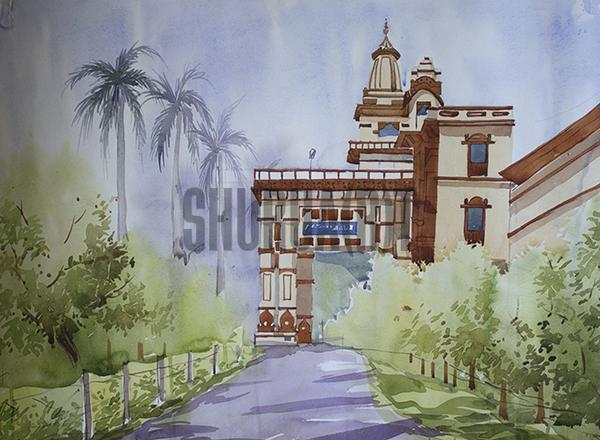
\includegraphics[width=\paperwidth,height=\paperheight]{./Banners/SketchPhysDept.jpg}} 
\begin{frame}[plain]

{\Large \color{red} Thanking you ! }

   \medskip

{\Large \color{white} Questions ?}
\end{frame}

\end{document}
